

\subsubsection*{Outline}
As previously stated, the methodology for cost-benefit analysis in water interventions had only been done on a local and selective fashion.
Thus, an approach that automated and generalized previous work was necessary.
This approach was based on the qualitative outline given by the World Health Organization from "Valuing Water, Valuing Livelihoods."
At it's core it focused on the ratio of benefits over costs in the form of Disability Adjusted Life Years gained over US Dollars.

\begin{equation}
\begin{aligned}
& \begin{matrix} \underline{\text{Years Gained}} \\ \text{Dollars} \end{matrix}
\end{aligned}
\end{equation}

Where Disability Adjusted Life Years are defined as:

\begin{equation}
\begin{aligned}
& \text{DALY} = (T \times n) + [(m \times d) + (D \times L)]\\
& T = \text{Travel time to water}\\
& n = \text{Trips to water per year}\\
& m = \text{Number of cases of diarrhea}\\
& d = \text{Days sick per case}\\
& D = \text{Death by diarrhea per year}\\
& L = \text{Average life expectancy}\\
\end{aligned}
\end{equation}

These variables were computed across a country in the assigned survey clusters and used a combination of data collection, standard industry values, and statistical inference.
The following will outline the order of the model's interaction.

\subsubsection*{Objective Function}
Let $X = \{X_1,X_2,X_3,...,X_n\}$ be the survey cluster locations and $y = \{y_1,y_2,y_3,y_4\}$ be the possible water interventions to help a cluster.
These are defined more specifically as:
\begin{equation}
\begin{aligned} 
& y_1 = \text{Chlorine filters}\\
& y_2 = \text{Hand Dug Well}\\
& y_3 = \text{Drilled Well}\\
& y_4 = \text{Communal Standpipe}\\
\end{aligned}
\end{equation}

Then, the objective statement for each $X_i$ rests as: %include per household somehow

\begin{equation}
\begin{aligned}
& \underset{y}{\text{maximize}}
& & \frac{T_y + S_y}{P_y}  \\
& T_y =
& & \text{Travel Time Gained from } y_i \\
& S_y =
& & \text{Illness and Death Time Gained from } y_i \\
& P_y =
& & \text{Cost of Intervention } y_i \\
\end{aligned}
\end{equation}

Each of these variables are dependent on various assumptions and approximate values.
Each will be broken down in turn.

\subsubsection*{Travel Improvements}
First, travel time gained is exclusive only to $y_2,y_3,y_4$ which contribute a new or improved water source.
In order to consider the location of the new intervention, various techniques were used to fill in the gaps of exact GPS locations for survey participants.
[Make sure data section covers this gap]
First, each region was split up into Voronoi shapes using survey cluster centers as the points of the diagram. %include Voronoi equation
The area of each shape was then computed by intersecting them with region boundaries and using the Shoelace or Gauss-Area formula. %include shoelace formula

%%% Include picture of sample Voronoi shapes in country or region boundaries %%%
\begin{figure}[h]
    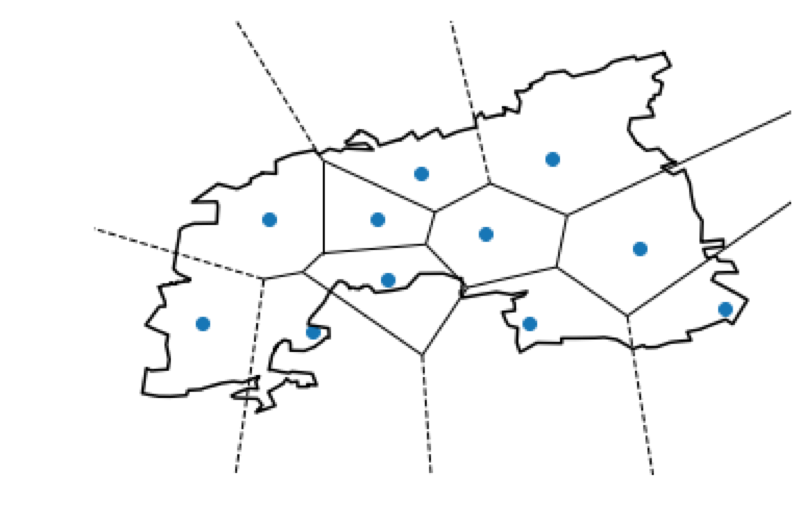
\includegraphics[width=\linewidth]{figures/voronoi.png}
    \caption{Sample Voronoi diagram within region.}
    \label{fig:voronoi}
\end{figure}

With this area found, a square shape was created with the same area and the surveyees were scattered throughout the square area using a uniform distribution and gamma distribution.
This scattering was based on the assumption that surveyees lived in clumps or population centers.

%%% Include picture of square with points scattered %%%
\begin{figure}[h]
    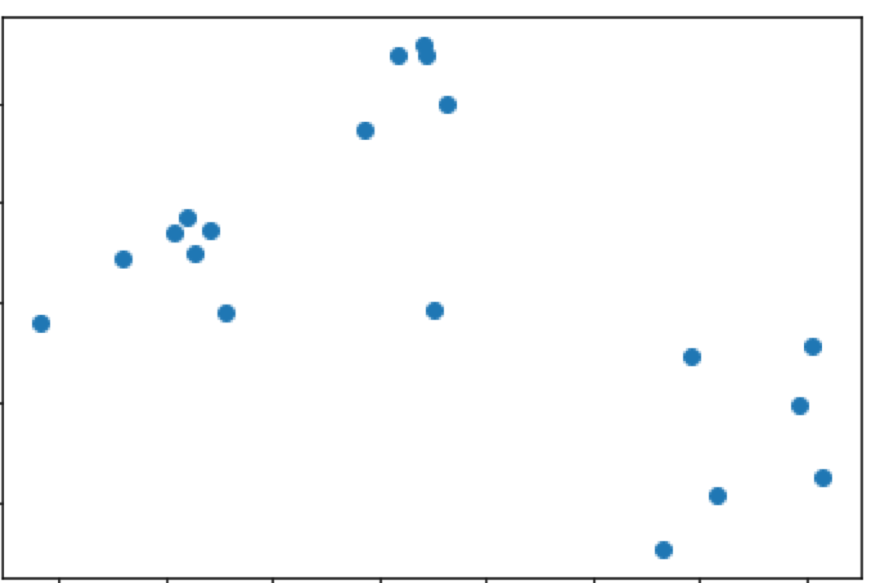
\includegraphics[width=\linewidth]{figures/clusters.png}
    \caption{Sample of cluster distribution per iteration.}
    \label{fig:clusters}
\end{figure}
A water source was then figuratively placed in the middle of our test area and each record was reviewed to see if it had an improved access to water, and how great the improvement was.
This process was performed over $G$ iterations and the results were recorded as $a_j$ for binary impact status and $b_j$ for the amount of impact:

%%%%%%%%%%%%%%%%%%%%%%%%
\begin{equation*}
\begin{aligned}
& a_j = \{a_{j1},a_{j2},...,a_{jG}\}\\\\
& a_{jg} =
\left\{
\begin{array}{ll}
      0 & \text{if impact}\\
      1 & \text{if no impact} \\
\end{array}
\right.\\\\
& b_j = \{b_{j1},b_{j2},...,b_{jG}\}\\\\
& b_{jg} =
\left\{
\begin{array}{ll}
      t_{\text{new}} - t_{\text{prev}} & \text{if impact} \\
      0 & \text{if no impact}\\
\end{array}
\right.
\end{aligned}
\end{equation*}

After $G$ iterations, the probability that each record would be affected in an intervention was given by:
\begin{equation*}
\frac{a_j}{G}
\end{equation*}
The approximate number of records affected in an intervention was given by:
\begin{equation*}
a = \sum_{j=1}^{J} \sum_{g=1}^{G} a_{jg}
\end{equation*}
The average impact on each of these records was recorded as
\begin{equation*}
\text{is this correct?}
b = \frac{\sum_{j=1}^{J} \sum_{g=1}^{G} b_jg}{a}
\end{equation*}

By this method, the improvement of travel time was quantified.

\subsubsection*{Illness and Death Improvements}
In addition to reducing the travel time to collect water, almost all listed interventions give also an improvement in health by reducing the cases of diarrhea in a country.
In order to calculate how many cases were reduced and how many years of life were gained by there reduction, values from the WHO and from the collected survey data were combined.

\subsubsection*{Cost of Intervention}
In order to get a cost of each intervention in $Y$, a great deal of standard values had to be used.
These costs had to be first divided into \emph{capital} and \emph{recurrent} costs.
Inflation had to be factored in and the following assumptions were made.
[Refer the constants that were assumed in the Appendix or define them here?]

$$c_1 = 20 \text{ (years each intervention lasted)}$$








